%\documentclass[a4paper]{article}
%\usepackage[utf8]{inputenc}
%\usepackage[spanish, es-tabla]{babel}
%\usepackage[table,xcdraw]{xcolor}
%\usepackage{amsmath}
%\usepackage{amsfonts}
%\usepackage{amssymb}
%
%\usepackage{float}
%\usepackage{graphicx}
%
%\usepackage{caption}
%\usepackage{subcaption}
%\captionsetup{compatibility=false}
%
%\usepackage{multirow}
%\setlength{\doublerulesep}{\arrayrulewidth}
%
%\newcommand{\quotes}[1]{``#1''}
%\newcommand\underrel[2]{\mathrel{\mathop{#2}\limits_{#1}}}
%
%\usepackage{array}
%\newcolumntype{C}[1]{>{\centering\let\newline\\\arraybackslash\hspace{0pt}}m{#1}}
%
%\usepackage[american]{circuitikz}
%\usepackage{xcolor}
%\usepackage{fancyhdr}
%
%\newlength{\stockheight}
%\usepackage{hyperref}
%
%\hypersetup{
%    colorlinks=true,
%    linkcolor=blue,
%    filecolor=magenta,      
%    urlcolor=blue,
%    citecolor=blue,    
%}
%
%\urlstyle{same}
%
%\usepackage{units} 
%\pagestyle{fancy}
%\fancyhf{}
%
%\rfoot{Página \thepage}

\subsection{Introducción}
En esta sección se implementó una compuerta \textbf{NOT} utilizando diversas tecnologías, siendo estas TTL (Transistor-Transistor-Logic), RTL (Resistor-Transistor-Logic) mediante transistores BJT (Bipolar Junction Transistor) y finalmente una variación de RTL utilizando un transistor MOSFET (Metal Oxide Semiconductor Field Efect Transistor).
\subsection{Comparación tecnologías.}
Usaremos dos tipos de transistores, siendo estos BJT y MOSFET.
\begin{itemize}
\item Los BJT son controlados por corriente, mientras que los MOS son controlados por tensión.
\item Los BJT tienen una respuesta mas veloz ante un cambio en su modo de funcionamiento\footnote{Saturación y corte} que los MOS dado a que poseen una menor capacidad.
\item Los transistores MOS tienen una mayor estabilidad frente a la temperatura que los BJT.	
\item Los transistores BJT cuentan con una corriente de polarización de base que los MOS no tienen ($I_g =0$).
\item La impedancia de entrada de los MOS es mucho mayor que la de los BJT.
\end{itemize}

\subsection{Circuitos Propuestos.}
Los circuitos propuestos son los siguientes:

\begin{figure}[H]
    \centering
    \begin{subfigure}[H]{0.3\textwidth}
        \centering
		\begin{circuitikz}
		\draw
		%%%%%%%%%%%%%%%%%%%%%
		%Figuras
		%%%%%%%%%%%%%%%%%%%%%
		node[npn](np1){}
		%%%%%%%%%%%%%%%%%%%%%
		%np1
		%%%%%%%%%%%%%%%%%%%%%
		(np1.E) to ++(0,-0.5)
			node[ground]{}
		(np1.B) to[R] ++ (-1.5,0)
			to[short,-o]++(-0.5,0)
			node[label=west:$V_{In}$]{}
		(np1.C) to [R,](0,2)
			to[short,-o]++(0,0.5)
			node[label= north:$V_{cc}$]{}
		(np1.C) to [short,-o]++(0.5,0)
			node[label = east:$V_{Out}$]{}
		;
		\end{circuitikz}

        \caption{RTL}
    \end{subfigure}%
    ~ 
      \begin{subfigure}[H]{0.3\textwidth}
        \centering
	\begin{circuitikz}
	\draw
	%%%%%%%%%%%%%%%%%%%%%
	%Figuras
	%%%%%%%%%%%%%%%%%%%%%
	node[nigfete](monch){}
	%%%%%%%%%%%%%%%%%%%%%
	%monch
	%%%%%%%%%%%%%%%%%%%%%
	(monch.S) to ++(0,-0.5)
		node[ground]{}
	(monch.G) to[R] ++ (-1.5,0)
		to[short,-o]++(-0.5,0)
		node[label=west:$V_{In}$]{}
	(monch.D) to [R,](0,2)
		to[short,-o]++(0,0.5)
		node[label= north:$V_{cc}$]{}
	(monch.D) to [short,-o]++(0.5,0)
		node[label = east:$V_{Out}$]{}
	;
	\end{circuitikz}
    \caption{RTL-MOS}
    \end{subfigure}%
    ~
    \begin{subfigure}[H]{0.39\textwidth}
        \centering
		\begin{circuitikz}
		\draw
		%%%%%%%%%%%%%%%%%%%%%
		%Figuras
		%%%%%%%%%%%%%%%%%%%%%
		node[npn,rotate=-90](np1){}
		(np1.C) to[open] ++(2,0)
		node[npn](np2){}
		%%%%%%%%%%%%%%%%%%%%%
		%np1, np2
		%%%%%%%%%%%%%%%%%%%%%
		(np1.E) to[short,-o] ++ (-1,0)
			node[label = west:$V_{In}$]{}
		(np1.B) to[R,-o] ++ (0,2)
			node[label = north:$V_{cc}$]{}
		(np1.C) -- (np2.B)
		(np2.C) to[R,-o]++(0,2)
			node[label = north:$V_{cc}$]{}
		(np2.C) to[short,-o] ++(0.5,0)
			node[label = east:$V_{Out}$]{}
		(np2.E) to[short] ++ (0,-0.5)
		node[ground]{}	
		;
		\end{circuitikz}
        \caption{TTL}
    \end{subfigure}
    \caption{Circuitos propuestos}
\end{figure}


\subsection{Diseño PCB.}
Se implementó en un único PCB los 3 circuitos, que corresponden al siguiente esquemático:
\begin{figure}[H]	
	\centering
	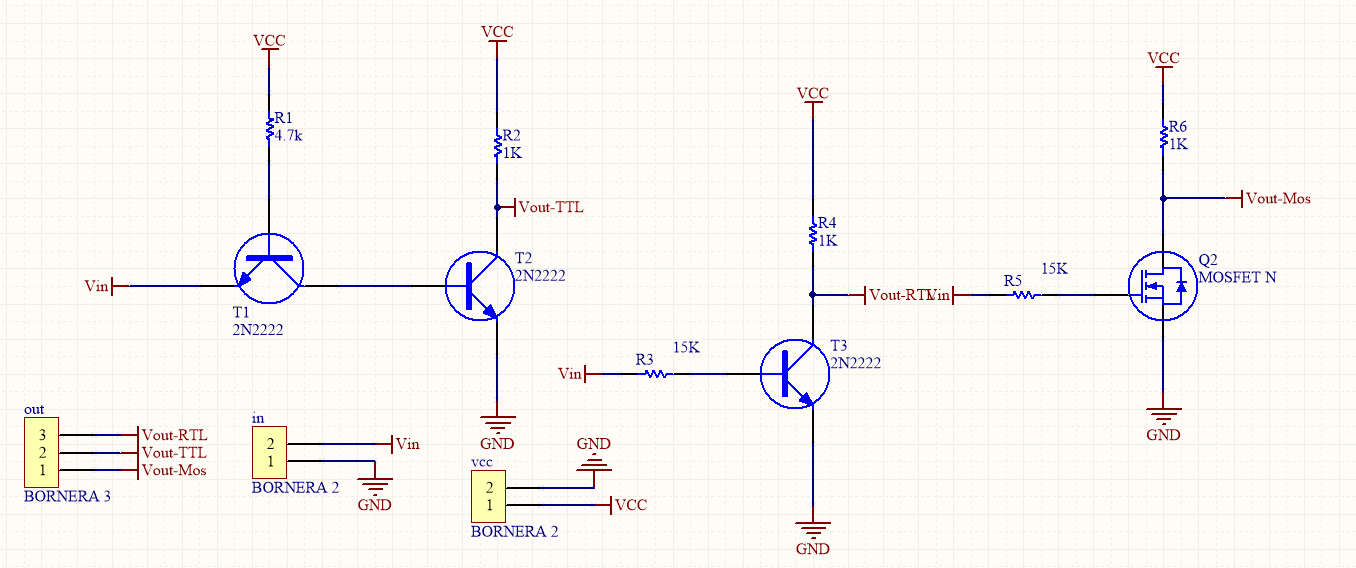
\includegraphics[width=0.5\textwidth]{Imagenes/Esquematico.PNG} \ \ \ \
	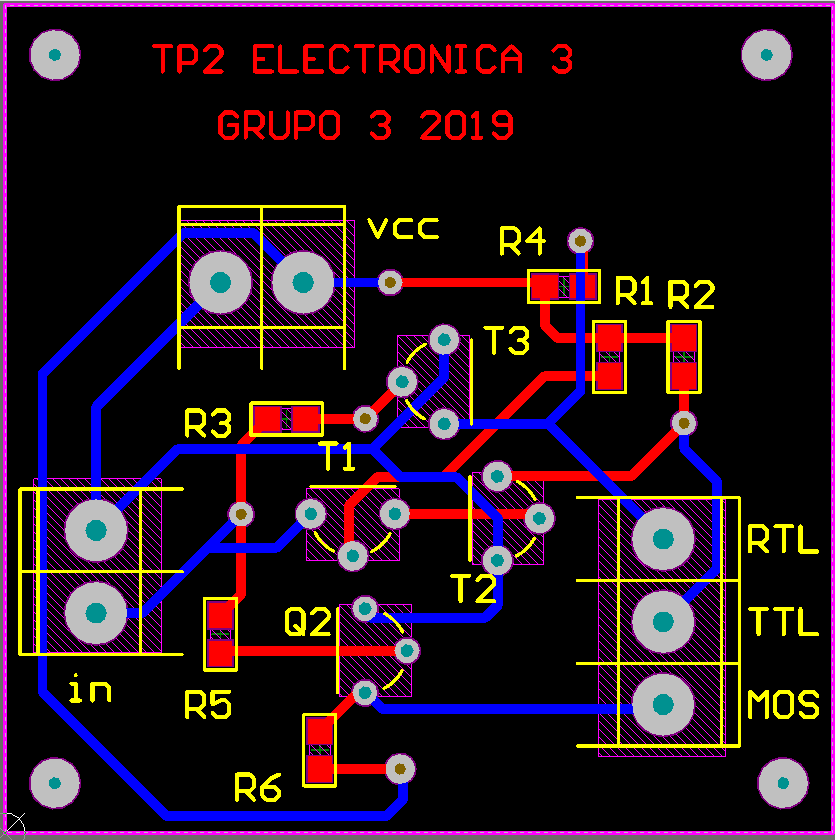
\includegraphics[width=0.3\textwidth]{Imagenes/PCB.PNG}
	\caption{Esquemático y PCB.}
	\label{fig:esquematico}
\end{figure}
%%%%%%%%%%%%%%%%%%%%%%%%%%%%%%%%%%%%%%%%%%%%%%%%%%%%%%%%

%%%%%%%%%%%%%%%%%%%%%%%%%%%%%%%%%%%%%%%%%%%%%%%%%%%%%%%%

\subsection{Observables de interés.}
\label{sec:Obs}
Se seleccionaron como observables de interés los siguientes parámetros:
\begin{enumerate}
\item \label{VIH} High-level input voltage 
\item \label{VIL} Low-level input voltage
\item \label{VOH}High-level output voltage
\item \label{VOL} Low-level output voltage
\item \label{NM}Noise Margin
\item \label{PHL}Popagation delay High to Low
\item \label{PLH}Popagation delay Low to High
\item \label{THL}Transition delay High to Low
\item \label{TLH}Transition delay Low to High
\item \label{MOC}Maximum output current
\end{enumerate}
Las mediciones de estos observables se realizaron de la siguiente manera. Para las mediciones de (\ref{VIH}), (\ref{VIL}), (\ref{VOH}), (\ref{VOL}) y (\ref{NM}) se utilizó una rampa la cual iba de un valor ligeramente inferior  a 0V  hasta 5 V, la razón de esto, es que dado a que se utilizó una rampa, contiene un salto en el cambio de periodos el cual contiene altas frecuencias y puede causar problemas, agregando ese pequeño tiempo en el cual la tenison es menor a 0V se alcanza a estabilizar la señal. La figura (\ref{fig:medramp}) es un ejemplo de una de las mediciones.
\begin{figure}[H]	
	\centering
	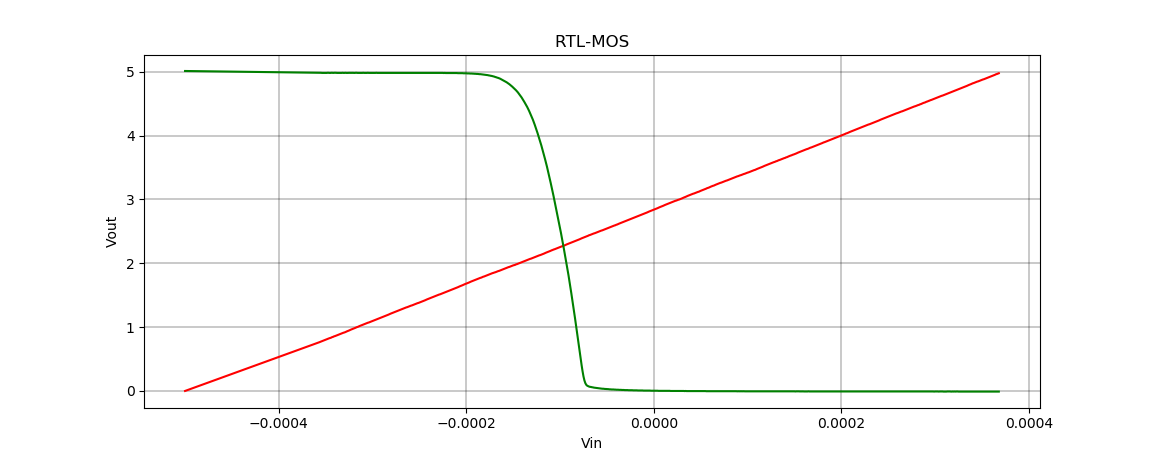
\includegraphics[width=0.9\textwidth]{Imagenes/DC-SWEEP/MedicionRampa.PNG}
	\caption{Medición niveles de tensión.}
	\label{fig:medramp}
\end{figure}
A partir de esta medición, se tomó el módulo de las señales y se graficó la señal de entrada en función de la salida, como se ve a continuación.
\begin{figure}[H]	
	\centering
	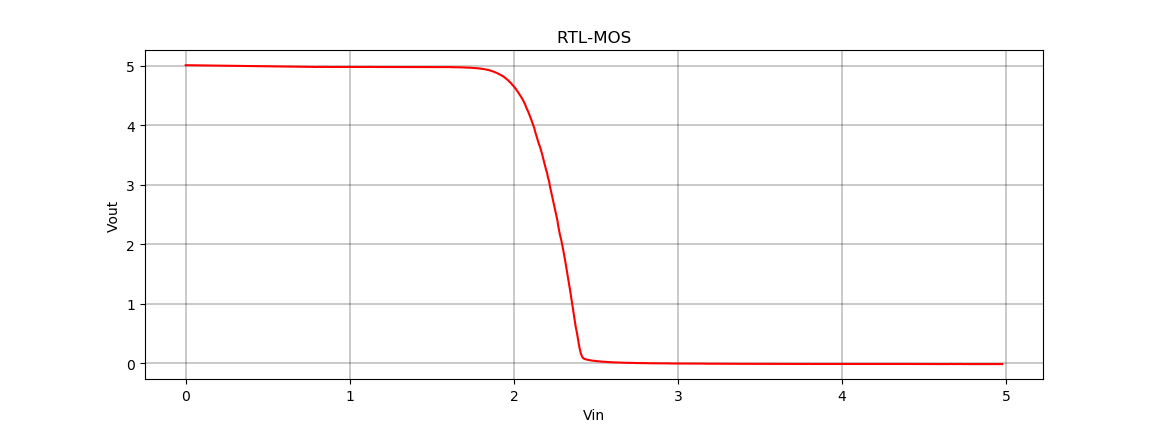
\includegraphics[width=0.9\textwidth]{Imagenes/DC-SWEEP/EntradaSalida.PNG}
	\caption{Medición entrada-salida.}
	\label{fig:medinout}
\end{figure}
finalmente a partir de esta imagen se buscó donde la pendiente es 45$^{\circ}$, de alli se obtuvo (\ref{VIH}), (\ref{VOH}), (\ref{VIL}) y (\ref{VOL}), realizando la resta de (\ref{VIH}) con (\ref{VOH}), y de (\ref{VIL}) con (\ref{VOL}) se obtienen los márgenes de ruido (\ref{NM}).

Luego para (\ref{PHL}),(\ref{PLH}),(\ref{THL}) y (\ref{TLH}) se midió la salida, con una cuadrada a la entrada como se ve en la siguiente figura:
\begin{figure}[H]	
	\centering
	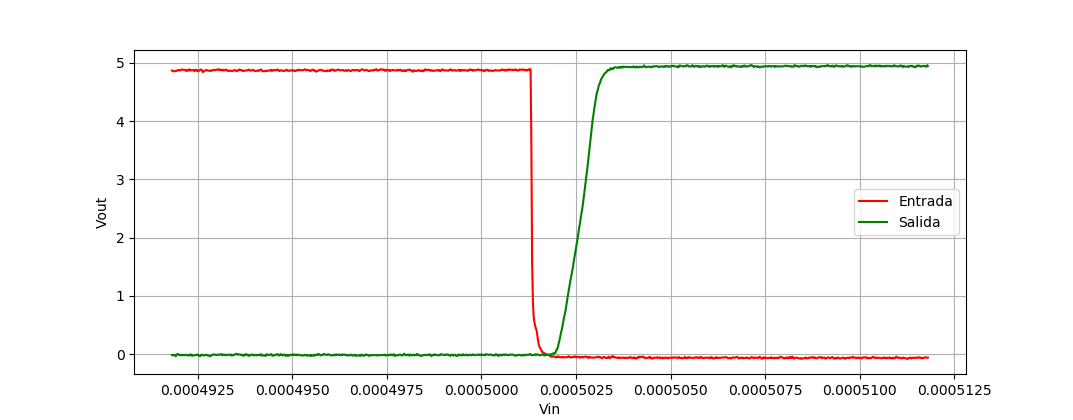
\includegraphics[width=0.9\textwidth]{Imagenes/DC-SWEEP/0t1mtl.PNG}
	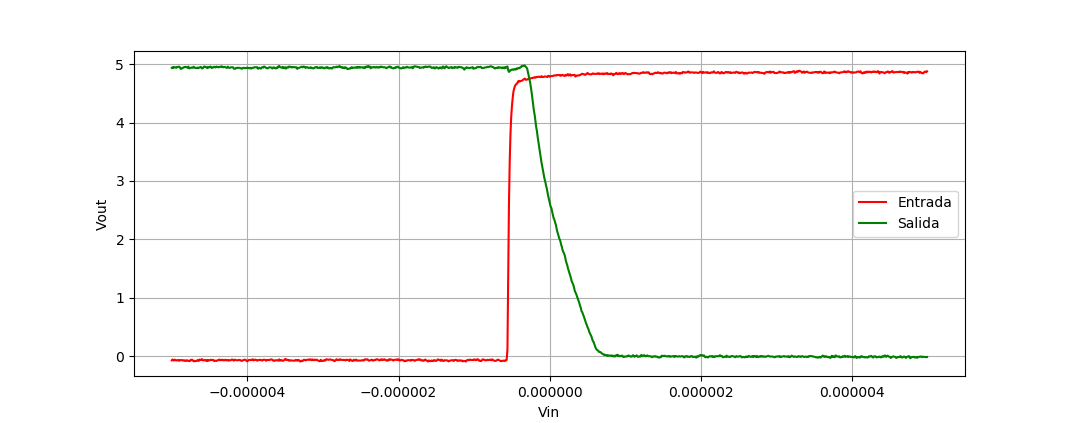
\includegraphics[width=0.9\textwidth]{Imagenes/DC-SWEEP/1t0mtl.PNG}
	\caption{Medición tiempo de propagación y transición.}
	\label{fig:MedicionTiempos}
\end{figure}
Tomando el tiempo de propagación medido al 50\% de la señal y el timpo de transición medido entre el 10 $\sim$ 90 \%. Para la medición del tiempo de propagación existe una medicion la cual dio un valor menor al tiempo de rise del osciloscopio, este resultado debe ser interpretado una cota del tiempo y no el valor exacto. 

Finalmente se colocó un trimmer de 50k$\Omega$ utilizandolo como  carga, se varió su impedancia hasta que el valor de tensión de la salida se encuentre por debajo del High Level output Voltage. A partir de este valor de tensión y la resistencia del trimmer, se obtiene la corriente máxima de salida.
\begin{figure}[H]	
	\centering
	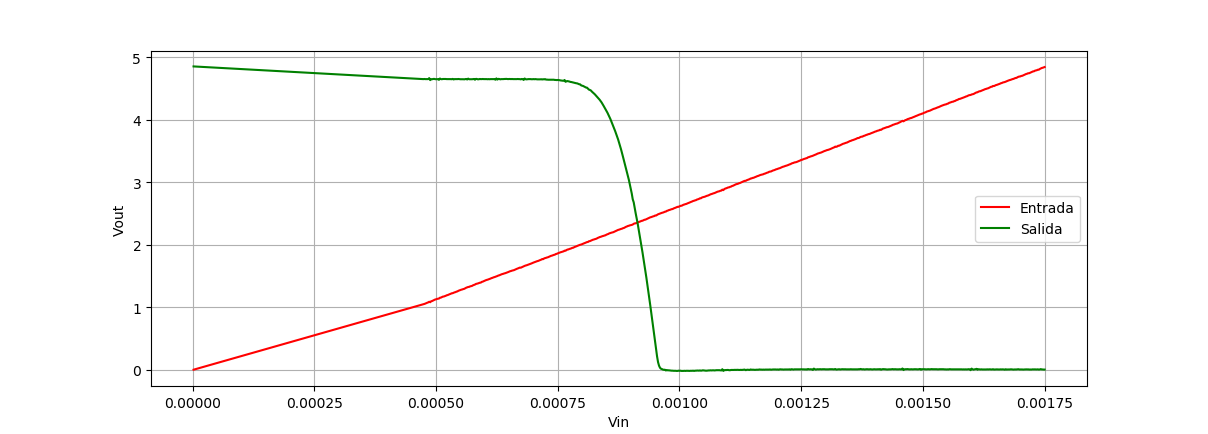
\includegraphics[width=0.9\textwidth]{Imagenes/DC-SWEEP/OutputCurrent.PNG}
	\caption{Medición corriente máxima de salida.}
	\label{fig:OutputCurrent}
\end{figure}

\subsection{Análisis de resultados.}
Para realizar una comparación entre los modelos propuestos, se utilizarán los observables de interés definidos en la sección (\ref{sec:Obs}) utlizando la siguiente tabla:
\begin{table}[H]
\centering
\begin{tabular}{c|ccc}
\hline
\multicolumn{4}{|c|}{\textit{Sin carga}}                                                                          \\ \hline
\multicolumn{1}{|c|}{\textbf{Tecnología}} & \textbf{RTL}   & \textbf{RTL-MOS} & \multicolumn{1}{c|}{\textbf{TTL}} \\ \hline
High-level input voltage                  & 864 mV         & 2.49 V           & 595 mV                            \\
Low-level input voltage                   & 454 mV         & 1.95 V           & 413 mV                            \\
High-level Output voltage                 & 4.96 V         & 4.89 V           & 4.96 V                            \\
Low-level Output voltage                  & 191 mV         & 72.1 mV          & 34.5mV                            \\
Noise Margin High                         & 4.01 V         & 2.34 V           & 4.37 V                            \\
Noise Margin Low                          & 263 mV         & 1.88 V           & 378 mV                            \\
Propagation delay High to Low             & 76.93 nS       & 569.51 nS        & 1.82 nS                           \\
Propagation delay Low to High             & 2.0489 $\mu S$ & 1.33 $\mu S$     & 535 nS                            \\
Transition delay High to Low              & 87.28 nS       & 734.4 nS         & 38.36 nS                          \\
Transition delay Low to High              & 605 nS         & 909 nS           & 307 nS                            \\
Maximum output current                    & 184.4  $\mu A$ &    217 $\mu A$              &                                  135.5$\mu A$ 	
\end{tabular}
\end{table}
%%%%%%%%%%%%%%%%%%%%%%%%%%%%%%
\begin{table}[H]
\centering
\begin{tabular}{c|ccc}
\hline
\multicolumn{4}{|c|}{\textit{Con carga}}                                                                         \\ \hline
\multicolumn{1}{|c|}{\textbf{Tecnología}} & \textbf{RTL}  & \textbf{RTL-MOS} & \multicolumn{1}{c|}{\textbf{TTL}} \\ \hline
High-level input voltage                  & 840 mV        & 2.48 V           & 627.5 mV                          \\
Low-level input voltage                   & 478.7 mV      & 2.01 V         &    490 mV                         \\
High-level Output voltage                 & 4.98 V        & 4.86 V          & 4.95 V                            \\
Low-level Output voltage                  & 278 mV        & 151 mV           & 72 mV                             \\
Noise Margin High                         & 4.14 V        & 2.52 V           & 4.32 V                            \\
Noise Margin Low                          & 200.7 mV      & 514.9 mV         & 417.3 mV                          \\
Propagation delay High to Low             & 260.7 nS      & 625.7 nS         & 33.6 nS                           \\
Propagation delay Low to High             & 2.615 $\mu S$ & 1.652 $\mu S$    & 1.216 $\mu S$                     \\
Transition delay High to Low              & 183.817 nS    & 417.19 nS        & 73.12 nS                          \\
Transition delay Low to High              & 2.691 $\mu S$ & 2.831 $\mu S$    & 2.687 $\mu S$                     \\
Maximum output current                    &  187.2 $\mu A$             &     216 $\mu A$             &   135.2 $\mu A$                               
\end{tabular}
\end{table}
 

Las diferencias entre los parámetros para las tres tecnologías son notables,
{\begin{center}\color{red} \begin{huge}
TOMI AUXILIO \end{huge} \rule{\linewidth}{0.5mm}\end{center} }